%% arara directives
% arara: xelatex
% arara: bibtex
% arara: xelatex
% arara: xelatex

%\documentclass{article} % One-column default
\documentclass[twocolumn, switch]{article} % Method A for two-column formatting

\usepackage{preprint}
\newcommand{\removelatexerror}{\let\@latex@error\@gobble}
%% Math packages
\usepackage{amsmath, comment, amsthm, amssymb, amsfonts, algorithm2e, algpseudocode, multicol,  graphicx, caption, subcaption, multirow}
\RestyleAlgo{ruled}
%\SetAlFnt{\scriptsize}
\graphicspath{ {./Pictures/} }
%% Bibliography options
\usepackage[numbers,square]{natbib}
\bibliographystyle{unsrtnat}
%\usepackage{natbib}
%\bibliographystyle{Geology}
%% General packages
\usepackage[utf8]{inputenc}	% allow utf-8 input
\usepackage[T1]{fontenc}	% use 8-bit T1 fonts
\usepackage{xcolor}		% colors for hyperlinks
\usepackage[colorlinks = true,
            linkcolor = purple,
            urlcolor  = blue,
            citecolor = cyan,
            anchorcolor = black]{hyperref}	% Color links to references, figures, etc.
\usepackage{booktabs} 		% professional-quality tables
\usepackage{nicefrac}		% compact symbols for 1/2, etc.
\usepackage{microtype}		% microtypography
\usepackage{lineno}		% Line numbers
\usepackage{float}			% Allows for figures within multicol
%\usepackage{multicol}		% Multiple columns (Method B)

\usepackage{lipsum}		%  Filler text

 %% Special figure caption options
\usepackage{newfloat}
\DeclareFloatingEnvironment[name={Supplementary Figure}]{suppfigure}
\usepackage{sidecap}
\sidecaptionvpos{figure}{c}

% Section title spacing  options
\usepackage{titlesec}
\titlespacing\section{0pt}{12pt plus 3pt minus 3pt}{1pt plus 1pt minus 1pt}
\titlespacing\subsection{0pt}{10pt plus 3pt minus 3pt}{1pt plus 1pt minus 1pt}
\titlespacing\subsubsection{0pt}{8pt plus 3pt minus 3pt}{1pt plus 1pt minus 1pt}

% ORCiD insertion
\usepackage{tikz,xcolor,hyperref}

\definecolor{lime}{HTML}{A6CE39}
\DeclareRobustCommand{\orcidicon}{
	
\begin{tikzpicture}
	\draw[lime, fill=lime] (0,0) 
	circle [radius=0.16] 
	node[white] {{\fontfamily{qag}\selectfont \tiny ID}};
	\draw[white, fill=white] (-0.0625,0.095) 
	circle [radius=0.007];
	\end{tikzpicture}
	\hspace{-2mm}
}
\foreach \x in {A, ..., Z}{\expandafter\xdef\csname orcid\x\endcsname{\noexpand\href{https://orcid.org/\csname orcidauthor\x\endcsname}
			{\noexpand\orcidicon}}
}
% Define the ORCID iD command for each author separately. Here done for two authors.
\newcommand{\orcidauthorA}{0000-0000-0000-0001}
\newcommand{\orcidauthorB}{0000-0000-0000-0002}
\newcommand{\orcidauthorC}{0000-0000-0000-0003}
\newcommand{\orcidauthorD}{0000-0000-0000-0004}

%%%%%%%%%%%%%%%%   Title   %%%%%%%%%%%%%%%%
\title{Parallel A* project}

% Add watermark with submission status
\usepackage{xwatermark}
% Left watermark
\newwatermark[firstpage,color=gray!60,angle=90,scale=0.32, xpos=-4.05in,ypos=0]{\href{https://doi.org/}{\color{gray}{Publication doi}}}
% Right watermark
\newwatermark[firstpage,color=gray!60,angle=90,scale=0.32, xpos=3.9in,ypos=0]{\href{https://doi.org/}{\color{gray}{Preprint doi}}}
% Bottom watermark
\newwatermark[firstpage,color=gray!90,angle=0,scale=0.28, xpos=0in,ypos=-5in]{*correspondence: \texttt{email@institution.edu}}

%%%%%%%%%%%%%%%  Author list  %%%%%%%%%%%%%%%
\usepackage{authblk}
\renewcommand*{\Authfont}{\bfseries}
\author{Lorenzo Ippolito, Mattia Rosso, Fabio Mirto}


%%%%%%%%%%%%%%    Front matter    %%%%%%%%%%%%%%
\begin{document}

\twocolumn[ % Method A for two-column formatting
  \begin{@twocolumnfalse} % Method A for two-column formatting  
\maketitle

\begin{abstract}
This project is part of System And Device Programming Exam (year 2022, Politecnico di Torino). The
goal was to implement one or more parallelized versions of the famous path searching A* (A star) algorithm.
It was requested us firstly to analyze the behaviour of the sequential version of A* with respect to the Dijkstra algorithm 
and secondly to implement a parallel version of A* to obtain results in terms of execution time, cpu usage and
memory usage. The results we have obtained were compared with the sequential version to understand
which can be the most effective approach to reach the initial goal.
\end{abstract}
%\keywords{First keyword \and Second keyword \and More} % (optional)
\vspace{0.35cm}

  \end{@twocolumnfalse} % Method A for two-column formatting
] % Method A for two-column formatting

%\begin{multicols}{2} % Method B for two-column formatting (doesn't play well with line numbers), comment out if using method A


%%%%%%%%%%%%%%%  Main text   %%%%%%%%%%%%%%%
%% %%%%%%%%%%%%%%%%%%%%%%% %%
%% CHAPTER 1: INTRODUCTION %%
%% %%%%%%%%%%%%%%%%%%%%%%% %%
\section{Introduction: about the A* algorithm}
A* is a graph-traversal and path-search algorithm. It is used in many contexts of computer science and 
not only. It can be considered as a general case of the Dijkstra algorithm. It is a Greedy-best-first-search algorithm that uses an heuristic function to guide
itself. What it does is combining:
\begin{itemize}
  \item \textbf{Dijkstra} approach: favoring nodes closed to the starting point(source)
  \item \textbf{Greedy-best-first-search} approach: favoring nodes closed to the final point(destination)
\end{itemize}
Using the standard terminology:
\begin{itemize}
  \item $g(n)$: exact cost of moving from source to $n$.
  \item $h(n)$: heuristic estimated cost of moving from a node $n$ to the destination.
  \item $f(n) = g(n) + h(n)$: combination of the actual cost with the estimated one.
\end{itemize}
At each iteration the node $n$ that has the minimum $f(n)$ is examinated(expanded).
\subsection{Heuristic design}
\paragraph{Premises} We are going to work with weighted oriented graphs where $V$ is the set on nodes/vertices
and $E$ is the set of edges of the form $(x,y)$ to indicate that an oriented edge from $x$ to $y$ exists and it
has weight indicated as $cost(x, y)$.
\paragraph{Heuristic properties} 
The heurstic function represents the acutal core of the A* algorithm. It represents a prior-knowledge that
we have about the cost of the path from every node (source included) to the destination. 
\begin{itemize}
  \item If we have not this prior information($h(n) = 0 \;\forall n \in V$) we are turning the A* algorithm into
        Dijkstra (this is why A* can be considered as a more general case of Dijkstra algorithm) but we always
        have the guarantee of finding the shortest path. 
  \item \textit{Admissible} Heuristic: if $h(n) < cost(n, dest) \;\forall n \in V$ (so the we never over-estimate the distance to
        get to the destination from a node $n$) A* will always find the shortest path and the heuristic
        function is called \textit{admissible}. The more inaccurate
        is the estimation the more nodes A* will need to expand (with the upper bound of expanded nodes
        if $h(n) = 0$).
  \item \textit{Consistent} Heuristic: if $h(x) \le cost(x, y) + h(y)$ for every edge $(x, y)$ (so the triangular
        inequality is always satisfied) A* has the guarantee of finding an optimal path without processing
        any node more than once. 
\end{itemize}
\paragraph{Corner cases} 
\begin{itemize}
  \item \textbf{Dijkstra}: As already discussed if $h(n)=0$ for every node in the graph A* turns into the Dijkstra algorithm.
  \item \textbf{Ideal}: We would obtain a perferct behaviour in case $h(n)$ is exactly equal to the cost of moving from $n$ to
  the destination (A* will only expand the nodes on the best path to get to the destination).
  \item \textbf{Full greedy-best-first search}: if $h(n) \gg g(n)$ than only $h(n)$ plays a role and A* turns into
        a completly greedy-best-first search algorithm.
\end{itemize}

%% %%%%%%%%%%%%%%%%%%%%%% %%
%% CHAPTER 2: APPLICATION %%
%% %%%%%%%%%%%%%%%%%%%%%% %%
\section{A* project application}
\paragraph{Problem definition} Given a wide range of fields where the A* algorithm can be applied we have choosed the one of
optimal path searching in geographical areas where the goal is to find the minimum distance path from a 
node source to a node destination.

\paragraph{Notation} We work with a weighted oriented graph $G$ that is made of nodes $n \in V$ that represent
road-realated points of interest and edges $(x,y) \in E$ represent unidirectional connections between these points.
Each edge $(x, y)$ is associated to a weight that is the great-circle distance between $x$ and $y$ measured
in meters.
\paragraph{Benchmark} We will exploit the DIMACS benchmark to make robust estimates of the designed algortithms.
Starting from the FIPS system format files provided we have adapted them (as better explained in section 3) to provide
to the algorithms a file containing information structured as:
\begin{itemize}
  \item Nodes: each node $n$ is defined as $(index, longitude, latitude)$ where $index$ is a natural progressive
        number starting from $0$ used to univocally identify the node and $(longitude, latitude)$ are the geographical
        coordinates of the node.
  \item Edges: each edge $(x, y)$ is defined as $(x, y, weight)$ and it represents a unidirectional connection
        from $x$ to $y$ (a road) with length $weight$ (great-circle distance from $x$ to $y$).
\end{itemize}
\subsection{Heuristic function: the great-circle distance}
As previoulsly discussed the A* algorithm needs an \textit{admssible} and \textit{consistent} heuristic to properly work and this
function is tipically problem-specific. Given the type of problem we are going to apply A* to we are going
to use a measure of geographical distance that extends the concept of heuclidean distance between two points:
the great-circle distance (that is the shortest distance over the earth surface measured along the
earth surface itself).
\begin{figure}[ht!]
  \centering
  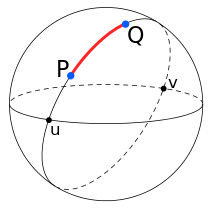
\includegraphics[width=0.5\linewidth]{others/haversine.png}
  \caption{Great circle distance from P to Q}
  \label{haversine}
\end{figure}
We will employee the \textbf{Haversine formula} to compute the distance from node $(\phi_1,\lambda_1)$
and node $(\phi_1,\lambda_1)$ where $\phi$ is the latitude and $\lambda$ is the longitude:
\begin{center}
  $d = R \cdot c$\\
  where $c = 2 \cdot atan2(\sqrt{a},\sqrt{1-a})$\\
  $a = sin^2\Big({\frac{\Delta \phi}{2}}\Big) + cos(\phi_1) \cdot cos(\phi_2) \cdot sin^2\Big({\frac{\Delta \lambda}{2}}\Big)$
  \\$R$ is the earth radius that we have fixed to $R=6.371km$
\end{center}

%% %%%%%%%%%%%%%%%%%%%%%% %%
%% CHAPTER 1: INPUT GRAPH %%
%% %%%%%%%%%%%%%%%%%%%%%% %%
\section{Graph file input}
\paragraph{File input format} 
Now we start discussing the A* algorithm implementation and to do that we need to specify which 
types of files we will need to provide to the algorithm to load the graph of interest. Each file has 
the format:
\begin{itemize}
    \item First line: the number of nodes $N[int]$
    \item N following lines: nodes appearing as $(index[int], longitude[double], latidue[double])$
    \item E following lines (with E unknown): edges appearing as $(x[int], y[int], weight[double])$
\end{itemize}
\paragraph{DIMACS benchmark} 
The benchmark files we have used come from the DIMACS benchmark. Here each geographic map is described by:
\begin{itemize}
  \item \textit{.co} file: a file containing the coordinates of the nodes following the FIPS system notation.
  \item \textit{.gr} file: a file containing the edges and the relative weight(distance) expressed in meters.
\end{itemize}
The generation of a file consistent with the format described above happens by merging these files 
into a new one (in binary format). One of the challenge we are going to undertake is the one of
parallelizing the reading of these huge files (that we will show having an high impact in terms of
execution time over the total time spent by the algorithm).
\paragraph{Test paths}
To analyze the performance of the different versions of A* algorithms we have used these paths:
\begin{table}[ht!]
	\caption{Test paths for A*}
	\centering
	\begin{tabular}{ |l|l|l|l| }
		\hline
		\textit{Nodes} & \textit{Edges} & \textit{Source} & \textit{Dest} \\ 
    \hline
		\multicolumn{4}{ |c| }{\bf{California(BAY)}} \\
		\hline
		\multirow{1}{*}{}
		321270& 800172 & 321269 & 263446\\
		\hline
		\multicolumn{4}{ |c| }{\bf{Florida(FLA)}} \\
		\hline
		\multirow{1}{*}{}
		1070376 & 2712798 & 0 & 103585\\
		\hline
    \multicolumn{4}{ |c| }{\bf{Western USA(W)}} \\
		\hline
		\multirow{1}{*}{}
		6262104 & 15248146 & 1523755 & 1953083\\
		\hline
    \multicolumn{4}{ |c| }{\bf{Full USA(USA)}} \\
		\hline
		\multirow{1}{*}{}
		23947347 & 58333344 & 14130775 & 810300\\
		\hline
	\end{tabular}
\end{table}
These paths have been chosen ad-hoc to make the algorithms find a way that crosses from side to side each one
of the these benchmark maps as showed in figure \ref{testpaths}.
\begin{figure}[ht!]
  \centering
  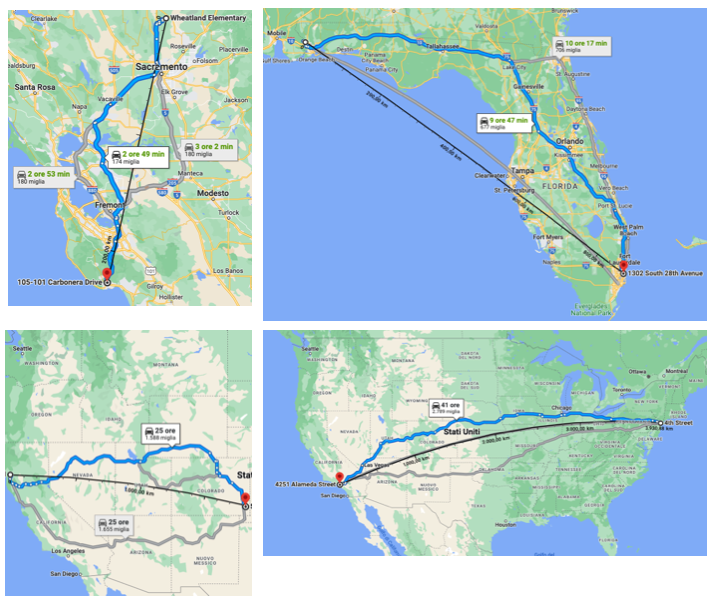
\includegraphics[width=0.8\linewidth]{others/google_maps.png}
  \caption{From left to right top to bottom BAY, FLA, W, USA}
  \label{testpaths}
\end{figure}

%% %%%%%%%%%%%%%%%%%%%%%%%% %%
%% CHAPTER 1: A* SEQUENTIAL %%
%% %%%%%%%%%%%%%%%%%%%%%%%% %%
\section{Sequential A* Algorithm}
Sequential A* algorithm is the one we will start with to see how it works and performs.
The first step consists of a pre-computation of:
\begin{itemize}
  \item The heurstic $h(n)$ for each node (by defintion $h(dest)$ will
        be 0) computed through the Haversine formula. We thus keep a data
        structure \texttt{h} to do this.
  \item The initial values of $f(n)$ and $g(n)$ that will be set to $DOUBLE\_MAX$ for each
        node except for the source node that will have $f(source) = h(source)$ because 
        $g(soruce)$ is clearly $0$. We thus keep data structures \texttt{f} and \texttt{g} to do this.
  \item The \textit{open set} contains all the nodes that still have to be explored(at
        the beginning only the source node).
  \item The \textit{closed set} contains all the nodes that have already been visited and don't
        have to be re-evaluated.
\end{itemize}
We will also need two additional data structures:
\begin{itemize}
  \item The \textit{costToCome} table (where \texttt{costToCome[i]} contains the current
        best cost to reach node \texttt{i}) that is initialized
        to $DOUBLE\_MAX$.
  \item The \textit{parentVertex} table (where \texttt{parentVertex[i]} contains the
        parent node of node \texttt{i} according to the current best path found to reach
        the destination) that is initialized with $-1$.
\end{itemize}
The outer loop is based on the nodes extraction from a \textit{open set}, the one containing
the nodes that have still to be explored (it is implemented as a Priory Queue where the priority
is associated to the $f(n)$ of the nodes). At each iteration the node $a$ with minimum $f(a)$ is
extracted from the \textit{open set} and its neighbors are expanded: the inner loop is repeated once for each neighbor $b$ of the
extracted node $a$($b$ is neighbor of $a$ if the edge $(a, b)$ exists). A tentative score is computed
for each node $b$ as $g(b) = g(a) + weight(a, b)$. If $g(b)$ is less than current \texttt{g[b]} these data structures
are updated: 
\begin{flushleft}
  \texttt{g[b] = g[a] + weight(a, b)}\\
  \texttt{costToCome[b] = g[b]}\\
  \texttt{parentVertex[b] = a}\\
  \texttt{f[b] = g[b] + h[b]}
\end{flushleft}
Since the heuristic function we have chosen is both \textit{admissible} and \textit{consistent} we have the guarantee 
that the first time a node is extracted from the \textit{open set} we have found a best path to it (this
is why when the destination node is extracted we can terminate having found the best path). So despite
one node may be added to the \textit{open set} more than once (when discovered as a neighbor of different nodes)
it will be expanded only one time.
\SetKwComment{Comment}{/* }{ */}
\begin{algorithm}[ht!] 
\caption{Sequential A*}\label{alg:two}
\KwData{Graph G(V,E), Source s, Destination d, Heurstic h}
\KwResult{Best path from Source to Destination and relative cost}
$g[i] \gets DOUBLE\_MAX \;\forall i \in V$\;
$f[i] \gets DOUBLE\_MAX \;\forall i \in V$\;
$h[i] \gets h(i, d) \; \forall i \in V$\;
$costToCome[i] \gets DOUBLE\_MAX \; \forall i \in V$\;
$parentVertex[i] \gets -1 \; \forall i \in V$\;
$f[s] \gets h[s]$\;
$g[s] \gets 0$\;
$openSet := \{(s, f[s])\}$\;
\While{$!openSet.EMPTY()$}{
  $a \gets openSet.POP()$\;
  \If{$a == d$}{
    $pathFound \gets true$\;
    reconstructPath()\;
  }
  \If{$a \in closedSet$}{
    CONTINUE
  }
  $closedSet.PUSH(a)$
  \ForEach{neighbor $b$ of $a$}{
    \If{$b \in closedSet$}{
      CONTINUE
    }
    $wt \gets weight(a, b)$\;
    $tentativeScore \gets g[a] + wt$\;
    \If{$tentativeScore$ is less than $g[b]$}{
      $parentVertex[b] \gets a$\;
      $costToCome[b] \gets wt$\;
      $g[b] \gets tentativeScore$\;
      $f[b] \gets g[b] + h[b]$\;
      $openSet.PUSH((b, f[b]))$\;
    }
  }
}
\end{algorithm}

\subsection{Results}
\begin{table}[ht!]
  \caption{Sequential reading + Sequential A* performance}
  \label{seqtimes}
  \begin{tabular}{|l|l|l|l|l|l|}
  \hline
  \textbf{}    & \textbf{File Size} & \textbf{Reading} & \textbf{A*} & \textbf{Total} & \textbf{\begin{tabular}[c]{@{}l@{}}Reading \\ Impact\end{tabular}} \\ \hline
  \textbf{BAY} & 20.51MB              & 0.9538s           & 0.2197s      & 1.1735s          & 81.3\%                                                         \\ \hline
  \textbf{FLA} & 69.09MB              & 3.1551s           & 0.7174s      & 3.8725s          & 81.5\%                                                           \\ \hline
  \textbf{W}   & 394.26MB             & 18.3065s          & 2.5890s      & 20.8955s         & 87.6\%                                                           \\ \hline
  \textbf{USA} & 1292.40MB            & 56.9942s          & 13.6716s     & 70.6658s         & 80.6\%                                                           \\ \hline
  \end{tabular}
\end{table}
We can realize from table \ref{seqtimes} (despite for the random graph that is too small to appreciate this result) that the 
reading time has a very high impact on the overall execution time of the algorithm and in section 6
we will investigate one technique for parallelizing the reading of the file. 
% %%%%%%%%%%%%%%%%%%%%%%%%% %
% CHAPTER 5: A* vs DIJKSTRA %
% %%%%%%%%%%%%%%%%%%%%%%%%% %
\section{A* and Dijkstra: a comparison}
As already mentioned the Dijkstra algorithm can be considered as a particular case of A* where we
don't have any prior knowledge about the distances beteween the nodes ($h(n) = 0 \;\forall n \in V$).
We have also seen that the more precise is the heuristic function we provide the less nodes the algorithm
will expand to get to the destination. To investigate this point we have run
Dijkstra algorithm on the same graph comparing the number of expanded nodes by the two algorithms:

\begin{table}[ht!]
  \caption{Expanded nodes in different maps}
  \begin{tabular}{|l|l|l|}
  \hline
  \textbf{} & \textbf{Dijkstra} & \textbf{Sequential A*}       \\ \hline
  \textbf{BAY}            & 318725 of 321270    & 157137 of 321270  \\ \hline
  \textbf{FLA}            & 996956 of 1070376   & 592480 of 1070376 \\ \hline
  \textbf{W}              & 5470394 of 1070376  & 1600083 of 1070376 \\ \hline
  \textbf{USA}            & 16676528 of 1070376 & 8998767 of 1070376 \\ \hline
  \end{tabular}
\end{table}
\begin{figure}[ht!]
  \centering
  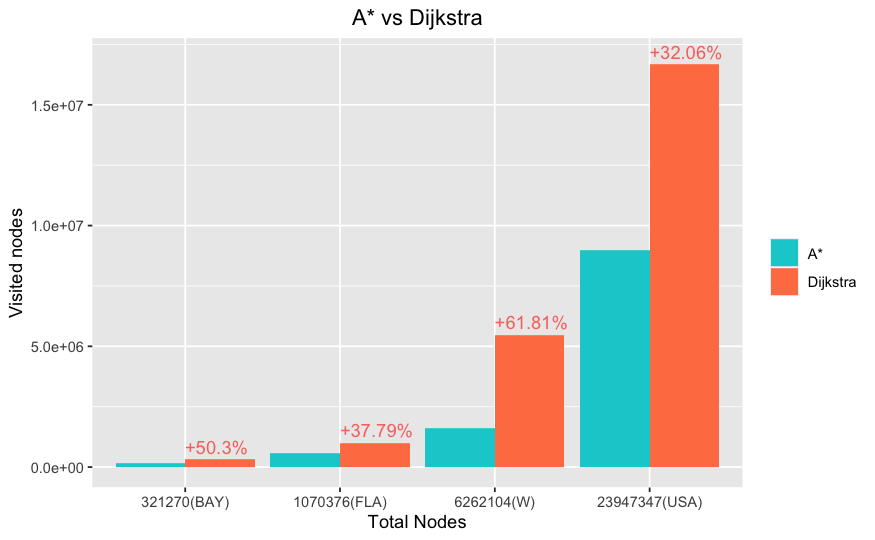
\includegraphics[width=1\linewidth]{astar_dijkstra/expanded_nodes.png}
  \caption{Expanded nodes: A* vs Dijkstra}
  \label{histogramnodes}
\end{figure}
The number of expanded nodes is clearly much higher when Dijkstra algorithm is used and the picture
\ref{astardijkstramap} cleary show in \textcolor{blue}{blue} the nodes expanded by the sequntial A* algorithm
while the \textcolor{red}{red} nodes are the ones expanded by the Dijkstra algorithm.
\begin{figure}[ht!]
  \centering
  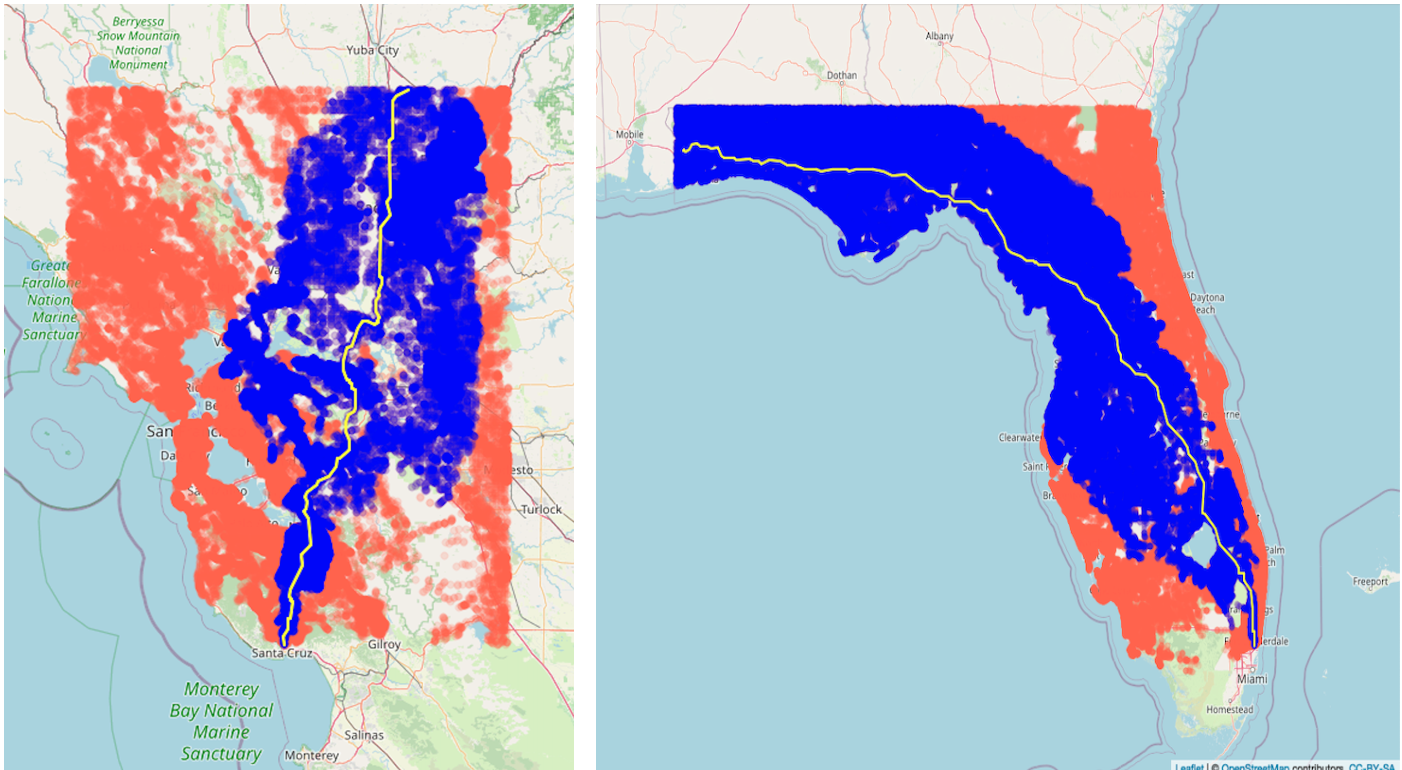
\includegraphics[width=1\linewidth]{astar_dijkstra/dijkstra_astar.png}
  \caption{Test paths on BAY(left) and FLA(right)}
  \label{astardijkstramap}
\end{figure}
In figure \ref{astardijkstratime} we can notice that the execution time is not necessary much better for A*.
This could depend both on the path we are looking for and on the precision of the heuristic function with
respect to the cost of the optimal path (in FLA map the heurist estimate is the point-to-point distance from
source to destination that is clearly different w.r.t. the actual best path). From figure \ref{astardijkstracpumem} we realize that considering 
CPU and Memory usage A* needs more memory
because of the higher number of data structures allocated but the less number of nodes expanded makes
the CPU usage inferior w.r.t Dijkstra algorithm in some cases.
\begin{figure}[ht!]
  \centering
  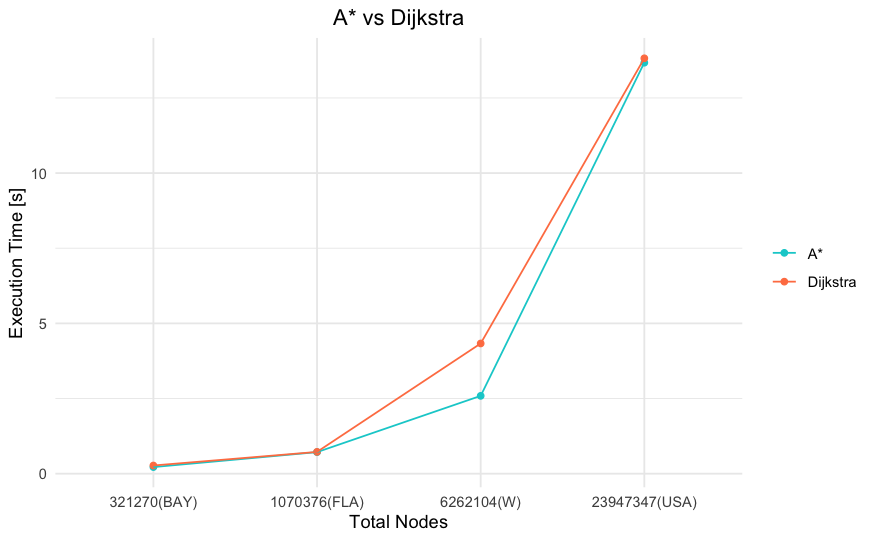
\includegraphics[width=1\linewidth]{astar_dijkstra/execution_time.png}
  \caption{Execution time: A* vs Dijkstra}
  \label{astardijkstratime}
\end{figure}
\begin{figure}[ht!]
  \centering
  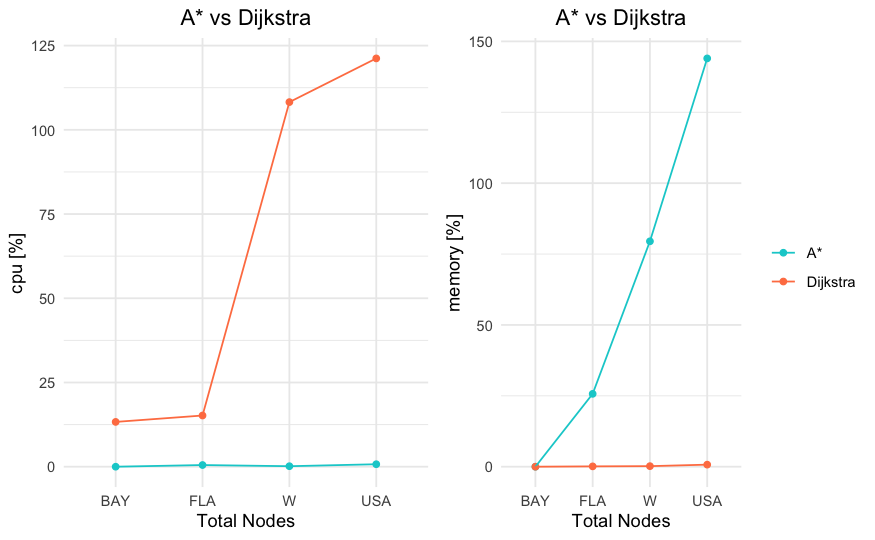
\includegraphics[width=1\linewidth]{astar_dijkstra/cpumem.png}
  \caption{Exploited resources: A* vs Dijkstra}
  \label{astardijkstracpumem}
\end{figure}
\section{Parallel reading of the input file}
As we have previously observed the time spent by the algorithm to read the input graph
(the input binary file) used by the A* algorithm is very high w.r.t. the total
amount of time. This is the reason why we have decided to inspect different techniques of
parallelization of the reading phase to speed it up (but only the explaied one prove
to be really effective). The input file, as already discussed,
is divided in two different sections (nodes and edges) so, in general, we need to take care of which
section a given thread is working on because different data structures of the graph need to
be loaded in the two sections (the symbol table when reading a \textit{node line} and the linked list when
reading a \textit{edge line}).
\begin{comment}
  \subsection{Parallel Read: approach 1}
In this first approach we have implemeted a solution on which:
\begin{itemize}
  \item $N$ threads runs freely to read the entire file
  \item Only one file descriptor is shared among all the threads (this means that
        when thread $t_i$ performs a \texttt{read} opearation all the other threads 
        are waiting for it to finish)
\end{itemize}
This is the most trivial solution that can be adopted and the drawback is the really high
resource contention that exists among all the threads (when N threads whant to access line
$k$ of the file only $1$ can do it and others $N-1$ wait). The advantage is that the file
will be read \textit{sequentially} but in a multithread fashion (line $k$ of the file
is always read before line $k+1$) and this results in a easier implementation.
\paragraph{Results on FLA}
\begin{figure}[ht!]
  \centering
  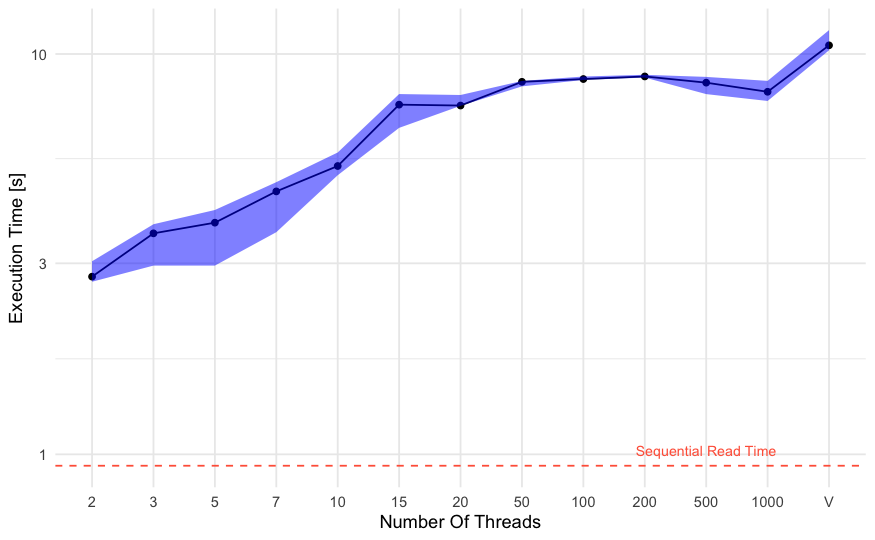
\includegraphics[width=1\linewidth]{par_read_1_time.png}
  \caption{Performance of approach 1 for different number of threads}
  \label{parread1time}
\end{figure}
\end{comment}
\subsection{Parallel Read: approach 1 (RA1)}
TODO how does it work
\paragraph{Results on FLA} 
As we can notice from figure \ref{parread2time} the most effective improvement comes probably from
the memory mapping. The increasing number of threads is infact not impacting well the reading time.
TODO why it happens
\begin{figure}[ht!]
  \centering
  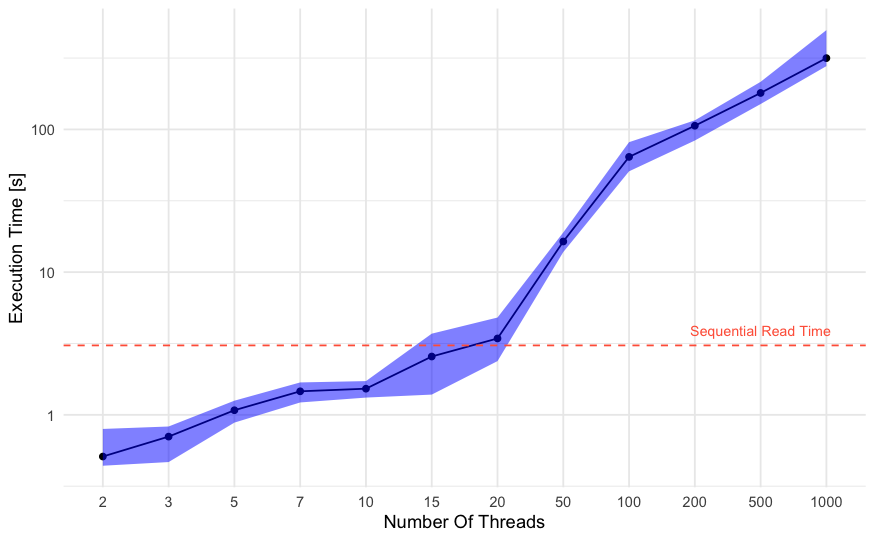
\includegraphics[width=1\linewidth]{read/par_read_1_time.png}
  \caption{Performance of RA1 for different number of threads on FLA}
  \label{parread1time}
\end{figure}
\begin{comment}
\subsection{Parallel Read: approach 3}
This is the approach is characterized by:
\begin{itemize}
  \item Letting threads differentiate among \textit{nodes section} and 
        \textit{edges section} to be able to read them togheter.
  \item Using a $(NP, NT)$ mechanism to read each section of the input file (where
        $NP$ is the number of partitions the section is divided in and $NT$ is the number
        of threads that have to read all the partitions).
\end{itemize}
\paragraph{The $(NP, NT)$ mechanism}
We need to provide as input:
\begin{itemize}
  \item $NP-nodes$: the number of partitions of the \textit{nodes section}
  \item $NP-edges$: the number of partitions of the \textit{edges section}
  \item $NT-nodes$: the number of threads that have to read the \textit{nodes section}
  \item $NT-edges$: the number of threads that have to read the \textit{edges section}
\end{itemize}
If the number of threads is equal to the number of partitions we have a simpler mechanism in
which each thread will read only one partition and then terminates.
As we can see in the example in figure \ref{parread3} threads will iterate over the partitions
of the sections that have been statically allocated to them. This means that there is not a real
contention of the reading phase since the partions are not overlapping and
each partition will be read by one and only one thread (actually, the
loading of the graph data structures after reading each line must be done in mutual exclusion so we will need a lock
both for the \textit{nodes-threads} and for the \textit{edges-threads}).
\begin{figure}[ht!]
  \centering
  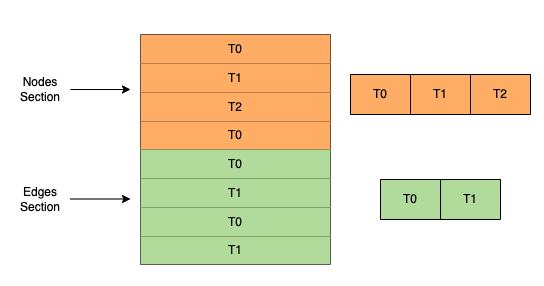
\includegraphics[width=1\linewidth]{read/par_read_3.png}
  \caption{Example of parallel read - approach 3}
  \label{parread3}
\end{figure}
Each thread terminates when it has no more partitions to read.\\
\paragraph{Results on FLA}
\begin{figure}[ht!]
  \centering
  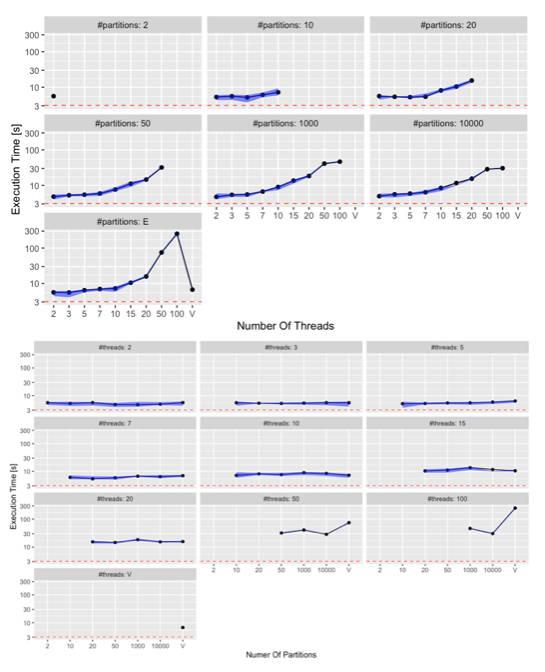
\includegraphics[width=1\linewidth]{read/par_read_3_time.png}
  \caption{Performance of approach 3 for different number of threads and partitions on FLA}
  \label{parread3time}
\end{figure}
We can realize from figure \ref{parread3time} that the number of partitions (setted equal
both for \textit{nodes section} and \textit{edges section}) has not a high impact.
What has more impact is the number of threads, an increasing number of threads gives increasing
bad performances while with a small number of threads we are able to obtain better results
w.r.t the first approach but worse result w.r.t the sequential reading. The reason of this
behaviour could be due to the fact that there is not a completly parallel work of the threads
since the access to Graph's data structure has to be done in mutual exclusion so we 
have benefits in dividing the threads in \textit{edges} threads and \textit{nodes} threads (something
that didn't happen in the first approach) but the mutual exclusion access to the Graph
makes the overhead due to threads creation and management not being able to obtain good
performances
\end{comment}
\subsection{Parallel Read: approach 2 (RA2)}
This parallel read approach is simply a variant of RA1. The only difference is that
instead of loading only the input graph $G$ it is also loaded the reversed graph $R$. This type of
reading is indeed applied only for using the PNBA* algorithm (more details in section later).
\begin{figure}[ht!]
  \centering
  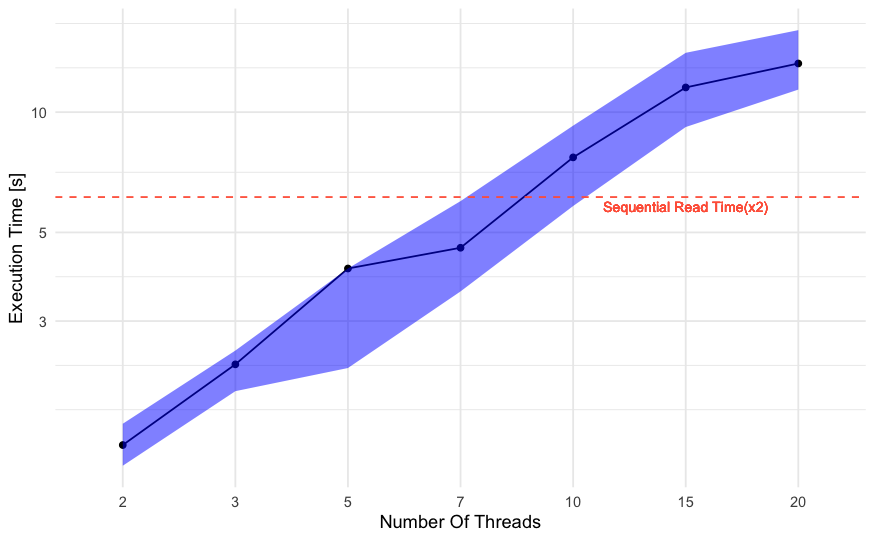
\includegraphics[width=1\linewidth]{read/par_read_2_time.png}
  \caption{Performance of RA2 for different number of threads on FLA}
  \label{parread2time}
\end{figure}
\subsection{Final results}
\begin{figure}[ht!]
  \centering
  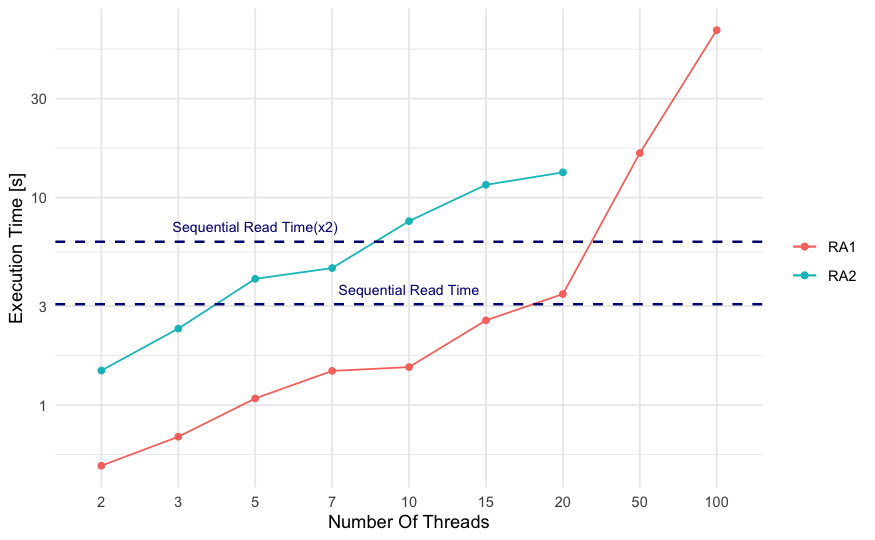
\includegraphics[width=1\linewidth]{read/par_read_all_time.png}
  \caption{RA(Read Approach) 1,2 compared with sequential reading on FLA - execution time}
  \label{parreadalltime}
\end{figure}
\begin{figure}[ht!]
  \centering
  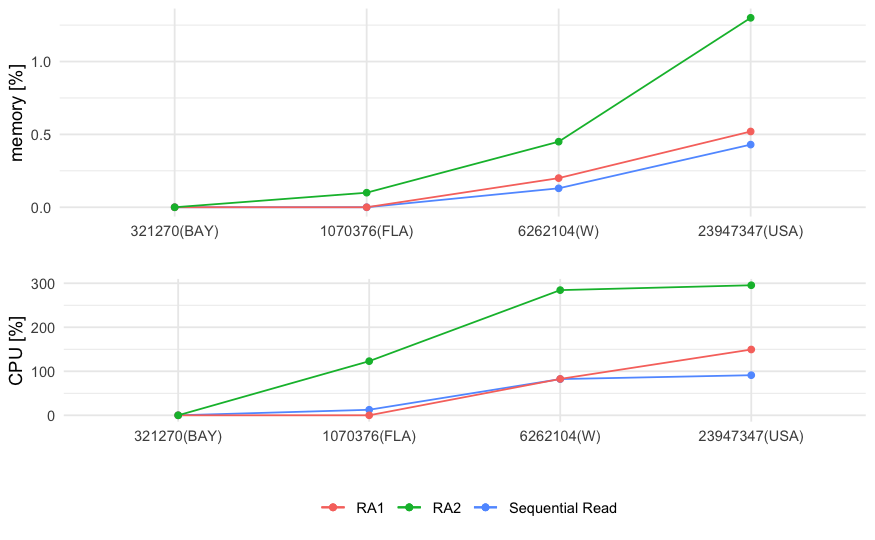
\includegraphics[width=1\linewidth]{read/parread_cpumem.png}
  \caption{RA(Read Approach) 1,2 compared with sequential reading on FLA - exploited resources}
  \label{parreadallcpumem}
\end{figure}
For the sake of completeness we have also test the most promising reading approach (RA1 and RA2 both with
2 threads) on all the maps (BAY, FLA, W, USA) and the results are showed in table \ref{readresultsfinal}
where the speed-up with respect to the sequential reading time is evident in particular for RA1.
\begin{table}[ht!]
  \centering
    \caption{RA1 results against sequential reading}
    \begin{tabular}{|l|l|l|l|}
    \hline
    \textbf{}    & \textbf{\begin{tabular}[c]{@{}l@{}}RA1\\ (2 threads)\end{tabular}} & \textbf{Sequential} & \textbf{Speed-Up} \\ \hline
    \textbf{BAY} & 0.1936s                                                            & 0.9366s             & 79.3\%            \\ \hline
    \textbf{FLA} & 0.5103s                                                            & 3.0650s             & 83.4\%            \\ \hline
    \textbf{W} & 3.3303s                                                              & 17.8834s            & 81.4\%            \\ \hline
    \textbf{USA} & 14.1492s                                                           & 56.4445s            & 74.9\%            \\ \hline
    \end{tabular}
    \label{readresultsfinal}
\end{table}

\begin{table}[ht!]
  \centering
    \caption{RA2 results against sequential reading}
    \begin{tabular}{|l|l|l|l|}
    \hline
    \textbf{}    & \textbf{\begin{tabular}[c]{@{}l@{}}RA2\\ (2 threads)\end{tabular}} & \textbf{Sequential(x2)} & \textbf{Speed-Up} \\ \hline
    \textbf{BAY} & 0.5313s                                                           & 1.8732s              & 71.6\%            \\ \hline
    \textbf{FLA} & 1.4682s                                                            & 6.1300s             & 76.1\%            \\ \hline
    \textbf{W} & 10.4959s                                                             & 35.7668s            & 70.7\%            \\ \hline
    \textbf{USA} & 35.4505s                                                           & 112.8890s            & 68.6\%            \\ \hline
    \end{tabular}
    \label{readresultsfinal}
\end{table}

\section{Parallel A*}
The goal of the project was to find one or more parallel versions of the A* algorithm 
and showing their performances w.r.t. the sequential version. We have choosen two approaches
to face the problem of parallelizing the A* algorithm: a first approach(known in literature as HDA*) that puts in action a
complex way of parallelizing the algorithm by defining a hash-based work distribution strategy and
a second approach that makes use of the parallelism in order to make the work of
finding the shortest path from \textit{source} to \textit{dest} split between only two threads
where one looks for the path from \textit{source} to \textit{dest} and the other one looks
for the path from \textit{dest} to \textit{source} in the reversed graph (the PNBA* algorithm).

\subsection{HDA*}
The Hash-Distributed-A* (HDA*) algorithm works is based on the fact that each thread is \textit{owner} of a
specific set of nodes of the Graph: given a node $n$ it is defined a hash function $f:\;f(n) = t$
where $t \in \{1..N\}$ with $N$ the number of threads. When a thread extracts from the \textit{open set}
(expands) a node all its neighbors are added to the \textit{open set} of the owner thread of the expanded node. 
One important fact is that HDA* doesn't provide the same guarantees of the sequential algorithm:
\begin{itemize}
  \item In sequential A* if it's provided an heuristic function that is both \textit{admissible}
        and \textit{consistent} we have the guarantee that each node will be only expanded once
        and that the first time we expand that node we have found a shortest path to it.
  \item In HDA* we loose these guarantees: since we don't know in which order nodes will be processed
        it could happen that a longer path to \textit{dest} is found before the shortest one so
        a node could be opened more than once and expanding the \textit{dest} node doesn't
        mean that we have terminated.
\end{itemize}
\paragraph{Hash Function}
The way how the threads divide among themself the work to be done happens using
a \textit{hash function}. The hash function that we have employeed at the 
beginning of our experiments was simply:
\begin{center}
  $hash_1(node\_index, num\_threads) = node\_index \;\%\; num\_threads$
\end{center}
As we can see in figure \ref{hdawork1} with 3 thread using this \textit{modulo} hash
function the work distribution is so equal
among the 3 threads that the way how each one works for finding an optimal path
to destination could be not the optimal one.
\begin{figure}[ht!]
  \centering
  \small
  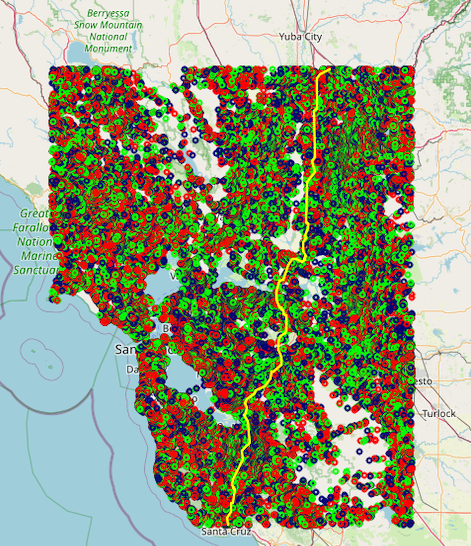
\includegraphics[width=0.5\linewidth]{hda/hda_work_BAY1.png}
  \caption{HDA* work distribution among 3 threads in BAY map (using $hash_1$ function)}
  \label{hdawork1}
\end{figure}
What proved to be a better approach was to employee another hash function that works in a different way:
\begin{center}
  $hash_2(node\_index, num\_threads, V) = i-1$\\[10pt]
  $i = min_i : \frac{V}{num\_threads}\cdot i > node\_index \;, i \in \{1,...,num\_threads\}$
\end{center}
What can be not optimal if we exploit the \textit{modulo} hash
function above could be that the fully randomly work distribution would make the work of each thread
much harder because lots of communication is needed and the termination condition is reached
many times with the result of more CPU consumption and time needed to find the solution. We can
define this as an absence of autonomy for each thread that causes a drastic communication
overhead. What tries to do the second hash function (the one that we have used to 
measure performances) is simply assigning nodes to threads following their index
numbering (e.g. nodes from $0$ to $K$ to thread $t_0$, nodes from
$K+1$ to $H$ to thread $t_1$ and so on and so forth). In this way we have tried to overcome
the limiations of the \textit{modulo} hash function. Different solutions that could be implemented in future works will be explained later.
\begin{figure}[ht!]
  \centering
  \small
  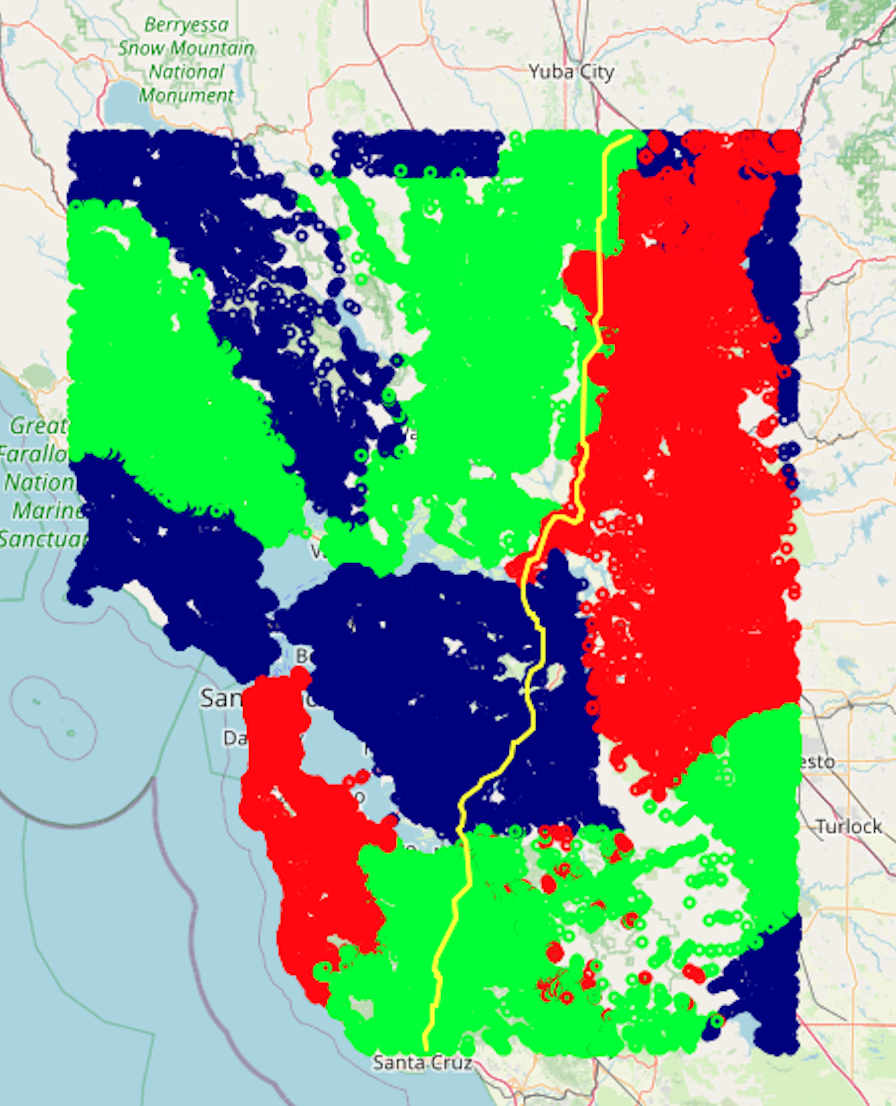
\includegraphics[width=0.5\linewidth]{hda/hda_work_BAY2.png}
  \caption{HDA* work distribution among 3 threads in BAY map (using $hash_2$ function)}
  \label{hdawork2}
\end{figure}
\paragraph{Distributed Termination Condition}
If in the sequential algorithm expanding the node \textit{dest} triggers the end of the algorithm (despite
the fact that the \textit{open set} could be not empty) in HDA* this is not valid anymore: when a thread
is working on its \textit{open set} it is expanding nodes putting their neighbors in the
\textit{open set} of another thread. When thread $t_i$ has its \textit{open set} empty it could think
to have finished its work but this might not be true because another thread $t_j$ could be sending
to $t_i$ some nodes that have to be be processed in the meanwhile. We have employed two
different approaches for the distributed termination condition that are:
\begin{itemize}
  \item \textbf{Barrier method (B)}: when a thread realizes that its \textit{open set} is
        empty a barrier is 
        hitten and when all the threads have hitten the barrier
        each one makes a check to confirm(or not) that all the \textit{open sets} of all
        the threads are still empty. If this is not true it means that there are nodes
        that have still to be processed and the best path to $dest$ found so far could
        not be the optimal one otherwise all the threads can terminate.
  \item \textbf{Sum-Flag method (SF)}: the idea behind the sum flag method comes from the fact that
        the Barrier mechanism could be quite expensive. In this termination condition method
        each thread keeps a binary flag saying whether its \textit{open set} is empty
        or not. When no more nodes are inside it the flag is set and if $\sum_{i=1}^{N}flag[i] = N$
        all the threads can correctly terminate.
\end{itemize}
\paragraph{Duplicate node checking}
The loose of guarantees explained before has also to do with the \textit{closed set} handling. In particular
when a node $n$ is expanded by thread $t_i$ it is done a check wheter this node is inside the \textit{closed set}
of thread $t_i$ or not. This is not sufficient: we also need to check whether the cost associated to that node 
when it was previously added to the \textit{closed set} is less or equal to the cost computed at the time $n$ is re-expanded. 
This is called duplicate checking so, a node $n$ is a duplicate of node $m$ if:
\begin{itemize} 
  \item $n$ is equal to $m$
  \item $closedSet$ of thread $t_i$ contains the node $m$
  \item $g(m) \le g(n)$
\end{itemize}
A duplicate node can be discarded.
\paragraph{Communication methodology}
What it differentiates the algorithms we have implemented is not only
the distributed termination condition (B or SF) but also the way how the threads
communicate with each other. This can be done using a shared address space (SAS) approach (that will
need to cope with mutual exclusion) or a message passing (MP) model.
\subsubsection{Message Passing Model (Using Message Queues) - MPMQ}
One way of achieving the communication among threads is message passing. In this first attempt we will rely
on Message Queues: when thread $t_i$ expands a node and computes(through the hash function) 
its owner $t_j$ a message is sent from $t_i$ to $t_j$. Since the message
queue is unique for all the threads each thread needs to be able to process
only messages directed to itself.  The termination condition that has been implemented in this case is the Barrier Method (B).
\paragraph{Data structures sharing}
Each thread mantains all the data structures as private (\textit{open set},
\textit{parentVertex}, \textit{costToCome}) and the only way it has communicate with other threads
is via message passing.
\paragraph{Message Structure} Each message sent from $t_i$ to $t_j$ regarding node $n$ contains:
\begin{itemize}
  \item Message id: the identifier of the owner thread $t_j$
  \item The index of the node $n$
  \item The parent node of $n$ (the one expanded from the \textit{open set} of $t_i$)
  \item The value of $g(n)$ according to $t_i$
  \item The value of $f(n)$ according to $t_i$
\end{itemize}
\paragraph{Message Based Path Reconstruction}
What it makes not trivial the path reconstruction phase in the Message Passing model
is that $parentVertex$ and $costToCome$ data structures are not shared among threads. 
This means that thread $t_i$ will have inside $parentVertex_i$, once the algorithm is terminated, 
a consistent value of $parentVertex_i[n]$ only for the nodes $n$ it is the owner of. This implies that if
we want to know which is the parent node of node $n$ in the final path this information
is stored in $parentVertex_i[n]$ (where $t_i$ is the parent of $n$). Path reconstruction needs to be done in a message passing fashion starting
from the destination's thread owner $t_d$. What happens is that $t_d$ sends a message to
the owner of $parentVertex_d[dest]$ (abbreviated as $pV_d[dest]$) that we call $t_k$. Immediately after $t_k$ will send a message
to $pV_k[pV_d[dest]]$ and so on and so forth till we have reached the first node of the path (the one with $pV_x[source] = -1$ where
$t_x$ is the owner of $source$).
\paragraph{Technical Issues}
Due to the fact that Message Queues have a limited size that is not enough to support any of our
selected benchmark graphs we have implemented the code but we weren't able to correctly test it. The
measures that will be reported next will only regard the MP model that exploits shared memory. 
\subsubsection{Message Passing Model (Using Shared Memory) - MPSM}
The Message Passing model that exploits Message Queues has been designed to work under the assumption 
that any data structure can be shared among threads. We are now going to relax this constraint by 
keeping some data structures shared among threads (like $parentVertex$ so that
the path reconstruction can happen in the standard way) and the exchange of messages will be based on Shared Memory.
\paragraph{Data structures sharing}
Each thread mantains some data structures as private (\textit{open set}...TODO) and the way how
a thread $t_i$ can send a node to be processed to its owner $t_j$ is by writing on Shared Memory. This
has the big advantage of minimizing the resource contention among threads (something that will strongly penalize the SAS model explained after).
\paragraph{Message Passing} Each message sent from $t_i$ to $t_j$ regarding node $n$ contains:
\begin{itemize}
  \item The index of the node $n$
  \item The parent node of $n$ (the one expanded from the \textit{open set} of $t_i$)
  \item The value of $g(n)$ according to $t_i$
\end{itemize}
The way how messages are read and written by the different threads is via \textit{Readers and Writers}
model where:
\begin{itemize}
  \item Thread writer $t_i$ writes on Shared Memory increasing a global pointer $p_G$.
  \item Thread reader $t_j$ reads from the Shared Memory by increasing a local pointer $p_j$. The reading
        of messages terminates when $p_j == p_G$.
\end{itemize}
\paragraph{Message Based Path Reconstruction}
Since the data structure $parentVertex$ is shared we no longer need message based path reconstruction.
\subsubsection{Shared Address Space Model}
This approach applies the explained concepts of HDA* by using a communication method
among threads that exploits the shared address space (SAS). There is:
\begin{itemize}
  \item A global array of \textit{open sets} that here we call $A$ where
        $A[i]$ contains a pointer to the \textit{open set} of thread $t_i$ and the size
        of $A$ is $N$ (the number of threads).
  \item The $parentVertex$ and $costToCome$ data structures are shared among all the threads.
\end{itemize}
This approach clearly requires locks so that the operations on the shared data structures
can happen in mutual exclusion. In particular we need:
\begin{itemize}
  \item One lock $L1$ for each \textit{open set} so for each $A[i] \;\forall i \in \{1..N\}$.
  \item One lock $L2$ for each node of the graph in order to correctly update $parentVertex$ and $costToCome$ data structures.
\end{itemize}
With SAS both the barrier (B) and the sum-flag (SF) distributed termination conditions
have been implemented to compare their performances.
\begin{comment}
\SetKwComment{Comment}{/* }{ */}
\begin{algorithm*}[] 
\caption{SAS-HDA*}\label{sas}
\KwData{Graph G(V,E), Source s, Destination d, Heurstic h}
\KwResult{Best path from s to d and relative cost}
\SetKwFunction{FMain}{HDAWrapper}
  \SetKwProg{Fn}{Function}{:}{}
  \Fn{\FMain{$source$, $dest$, $N$, $heuristic$}}{
        $g[i] \gets DOUBLE\_MAX \;\forall i \in V$\;
        $h[i] \gets heuristic(i, dest) \; \forall i \in V$\;
        $parentVertex[i] \gets -1 \; \forall i \in V$\;
        $t\_owner \gets hash(source, num\_threads)$\;
        $f[t\_owner][source] \gets h[s]$\;
        $g[source] \gets 0$\;
        $openSet[t\_owner] := \{(source, f[t\_owner][source])\}$\;
        Initialize $N$ $mutex\_threads$\;
        Initialize $V$ $mutex\_nodes$\;
        Launch $N$ threads\;
        Join $N$ threads\;
        Reconstruct final path\;
        \KwRet\;
}
\SetKwFunction{FHDA}{HDA}
  \SetKwProg{Fn}{Function}{:}{}
  \Fn{\FHDA{$index$, $dest$, $N$, $heuristic$}}{
    \While{$1$}{
      \While{$!openSet[index].EMPTY()$}{
        LOCK($mutex\_threads[index]$)
        $a \gets openSet.POP()$\;
        UNLOCK($mutex\_threads[index]$)
      }
      \If($a$ is duplicate){
        continue\;
      }
      \ForEach{neighbor $b$ of $a$}{
        $wt \gets weight(a, b)$\;
        $tentativeScore \gets g[a] + wt$\;
        \If{$tentativeScore$ is less than $g[b]$}{
          $owner\_a \gets hash(a,N)$\;
          $owner\_b \gets hash(b,N)$\;
          \If($b$ is duplicate){
            continue\;
          }
          LOCK($mutex\_nodes[a]$)
          $tentativeScore \gets g[a] + wt$\;
          UNLOCK($mutex\_nodes[a]$)

          LOCK($mutex\_nodes[b]$)
          \If{$tentativeScore$ is less than $g[b]$}{
            $parentVertex[b] \gets a$\;
            $costToCome[b] \gets wt$\;
            $g[b] \gets tentativeScore$\;
            $f[b] \gets g[b] + h[b]$\;
            LOCK($mutex\_threads[owner\_b]$)
            $f[owner\_b][b] \gets f[b]$\;
            $openSet.PUSH((b, f[b]))$\;
            UNLOCK($mutex\_threads[owner\_b]$)
          }
          UNLOCK($mutex\_nodes[a]$)
        }
      }

      \If{$openSet[index].EMPTY()$ and $parentVertex[b] != -1$}{
        Terminate according to B or SF\;
      }
    }
        \KwRet\;
}
\end{algorithm*}
\end{comment}
\subsection{Results}
In table \ref{tablesas} we have only inserted data related to SAS method with SF termination condition.
\begin{table}[ht!]
  \centering
  \caption{SAS-SF with best number of threads time performances}
  \begin{tabular}{|l|l|l|l|l|}
  \hline
  \textbf{}    & \textbf{Threads} & \textbf{SAS-SF} & \textbf{Sequential A*} & \textbf{Slow-Down}\\ \hline
  \textbf{BAY} & 5        & 0.5097s                & 0.2647s  &92.6\%          \\ \hline
  \textbf{FLA} & 7        & 1.6383s                & 0.7174s  & 128.3\%          \\ \hline
  \textbf{W}   & 7        & 10.8626s                & 2.5890s &319.6\%           \\ \hline
  \textbf{USA} & 7         & 30.5655s               & 13.6716 &123.6\%           \\ \hline
  \end{tabular}
  \label{tablesas}
\end{table}
These are the troubles found during implementation and testing:
\begin{itemize}
  \item The SAS-MP variant of HDA* is not scalable. This is due to the fact that we
        have used Linux Message Queues that have a limited size (few bytes) and when
        the communication overhead becomes huge the queue gets full causing a impressive
        slowdown.
  \item The SAS HDA* that exploits the Barrier termination condition (SAS-B) is more scalable
        than SAS-MP but the termination condition is not well-performing in large graphs. This 
        happens because a thread has no way to shortcut the barrier if it's receiving work from
        another thread but it has to wait until all the threads have reached the barrier. Despite
        the fact that we notice an improvement when the number of threads increases the execution
        time degenerates when using maps W and USA.
  \item The SAS HDA* that exploits the Sum-Flag termination condition (SAS-SF) behaves overall better.
        Despite the fact that on maps BAY, FLA, W it is difficult to notice the improvements when
        the number of threads increases this is more evident on USA map. Performances are always
        better compared to the SAS-B algorithm.
  \item About the resource consumption both SAS-B and SAS-SF are more expensive in terms on CPU and 
        memory used w.r.t the sequential algorithm. The resource used increase as the number of threads
        increase.
\end{itemize}
HDA* has been proven not to work well in our application. We have tried to explain these 
results by observing that:
\begin{itemize}
  \item The hash function has an important impact on the performances of A* algorithm. The one that
        we have used is probably not the optimal(for instance tring to assign near nodes
        to the same threads maybe by pre-clustering the nodes of the map in a number of clusters
        equal to the number of threads could be a better option). This could lead to obtain better performances but we
        suppose that the sequential algorithm would still be the "best case" instead of being the "worst case"
        in terms of execution time. 
  \item The termination condition is clearly a bottleneck, in particular if the Barrier method
        is used. This can be less evident with small maps but we can appreciate it on bigger graphs.
        By increasing the number of threads both SAS-SF and SAS-B perform better in terms of execution time even if
        the resource consumption increases but this is not enough and the performances scalability
        and improvements that should have been obtained with large graphs were not proved.
\end{itemize}
\subsection{New Bidirectional A*(NBA*)}
The NBA* algorithm is a version of  the bidirectional search that uses a data
structure $M$ to keep track of the nodes in the middle between the two searcher
threads $t_G$ and $t_R$. $M$ initially contains all the nodes of the graph. The nodes
in the search frontiers are the ones that:
\begin{itemize}
  \item Belongs to $M$
  \item Have been labelled: $g_G(n) < \infty $ or $g_R(n) < \infty $
\end{itemize}
The threads $t_G$ and $t_R$ share a variable $L$ initialized to $\infty$ that contains
the cost of the best path from $source$ to $dest$. Other common variables are:
\begin{itemize}
  \item $F_G$: lowest $f_G$ value on $t_G$ frontier.
  \item $F_R$: lowest $f_R$ value on $t_R$ frontier.
  \item Variables $F_p$, $f_p$, $g_p$ (with $p \in \{R,G\}$) are written on only one
        side but read by both sides.
\end{itemize}
These are the initialization steps done by $t_G$ (same for $t_R$)
\begin{itemize}
  \item $g_G(source_G)=0$, $F_G(source_G)=f_G(source_G)$
\end{itemize}
At each iteration it is extracted a node $x$ such that:
\begin{itemize}
  \item $x \in M$
  \item $x: f_G(x) = min f_G(v) \forall v \in openSet_G$ 
\end{itemize}
The node is removed from $M$ and pruned (not expanded) if $f_G(x) \ge L$ or
$g_G(x)+F_R-h_R(x) \ge L$. Otherwise all its successors $y$ are generated. In the
first case it is classified as \textit{rejected} while in the other situation it is
\textit{stabilized} because $g_G(x)$ won't be changed anymore. For each $y$ we update:
\begin{itemize}
  \item $g_G(x)$: $min(g_G(y), g_G(x) + d_G(x, y))$
  \item $L$: $min(L, g_G(x) + g_G(y))$
\end{itemize}
The algorithm stops when no more candidates have to be expanded in one of the two sides.
\subsection{Parallel New Bidirectional A*(PNBA*)}
The PNBA* algorithm improves the NBA* algorithm by letting the two threads working in
parallel and not in a alternate mode. This requires to cope with mutual exclusion on some data.
\begin{figure}[ht!]
  \centering
  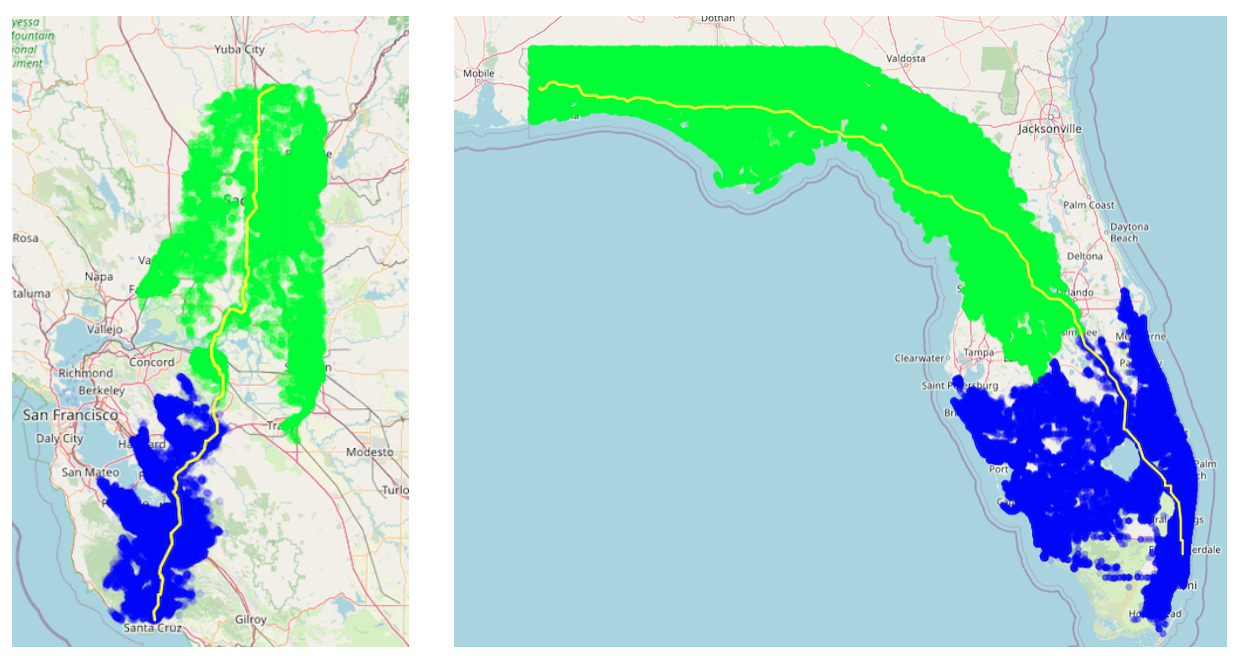
\includegraphics[width=1\linewidth]{pnba/pnbamap.png}
  \caption{PNBA* work on BAY(left) and FLA(right)}
  \label{pnbamap}
\end{figure}
In figure \ref{pnbamap} we realize that the work distribution is not equal and changes 
at each iteration (depending on which is the common node found).
\subsubsection{Results}
\begin{table}[ht!]
  \centering
  \caption{PNBA* - time performances}
  \begin{tabular}{|l|l|l|l|}
  \hline
  \textbf{}    & \textbf{PNBA*} & \textbf{Sequential A*} & \textbf{Speed-Up} \\ \hline
  \textbf{BAY} & 0.2091s        & 0.2197s                & 4.82\%            \\ \hline
  \textbf{FLA} & 0.6782s        & 0.7174s                & 5.46\%            \\ \hline
  \textbf{W}   & 2.3029s        & 2.5890s                & 11.1\%            \\ \hline
  \textbf{USA} & 9.0568         & 13.6716s               & 33.8\%            \\ \hline
  \end{tabular}
\end{table}
\begin{itemize}
  \item The PNBA* is able to outperform the sequential algorithm in terms of execution time in all the 
        graphs we have tested it on. The speed-up increases as the number of nodes increases and this can 
        be a good news if we will try to implement it on much bigger graps. The execution time and the number of
        nodes have been proved to strongly depend on the position of the common node found. Best performances
        are achieved when the common node found is approximately in between of source and destination nodes.
  \item Resource consumption is almost 2x w.r.t. the sequential algorithm and this is reasonable considering
        that it is like running two sequential algorithm in concurrency
\end{itemize}
\section{Computing Facilities Platform}
We have tested all our work on the \textit{SmartData@PoliTO} Cluster.
There are $33$ storage workers equipped with:
\begin{itemize}
  \item 216 TB of raw disk storage
  \item 384 GB of RAM
  \item Two CPUs with 18 cores/36 threads each
  \item Two 25 GbE network interfaces
  \item More than 50 GB/s of data reading and processing speed
\end{itemize}

\section{Future Work}
(Possible improvements)

\section{Complete Results}
\begin{center}
  \begin{figure}[ht!]
    \centering
    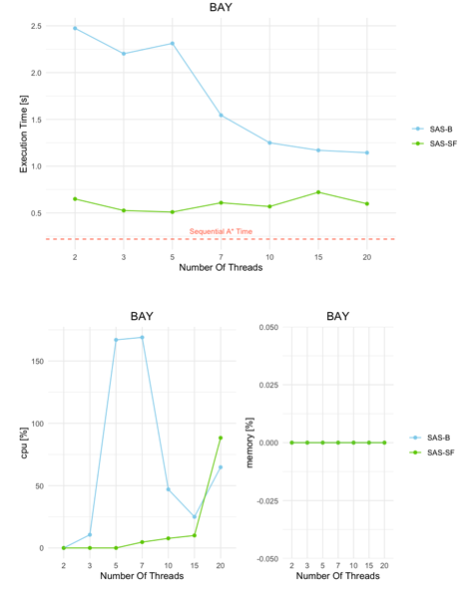
\includegraphics[width=1\linewidth]{hda/bay.png}
    \caption{HDA* on BAY map}
    \label{hdabay}
  \end{figure}
\end{center}
\begin{figure}[ht!]
  \centering
  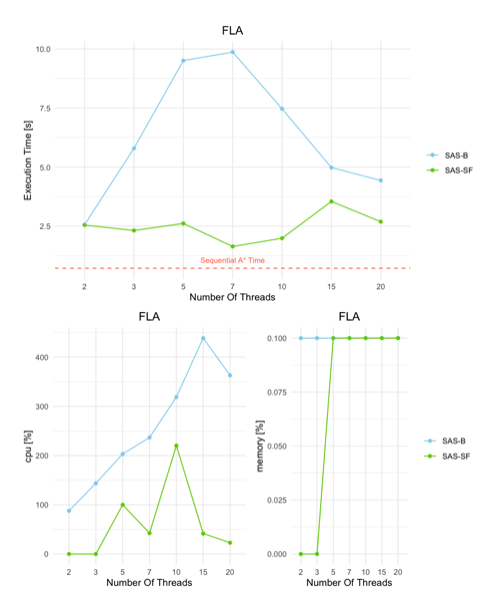
\includegraphics[width=1\linewidth]{hda/fla.png}
  \caption{HDA* on FLA map}
  \label{hdafla}
\end{figure}
\begin{figure}[ht!]
  \centering
  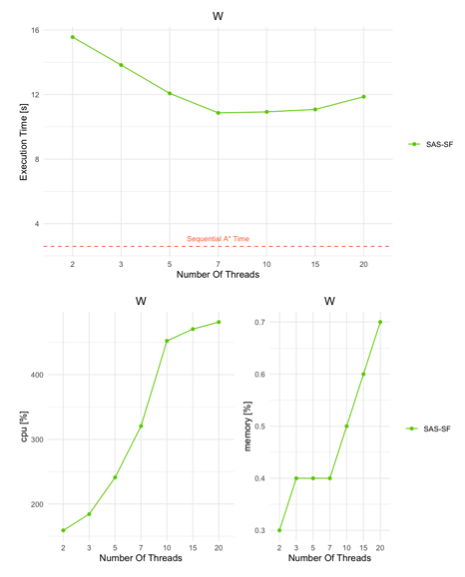
\includegraphics[width=1\linewidth]{hda/w.png}
  \caption{HDA* on W map}
  \label{hdaw}
\end{figure}
\begin{figure}[ht!]
  \centering
  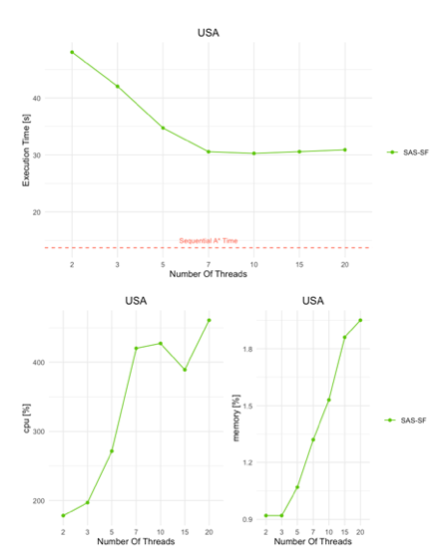
\includegraphics[width=1\linewidth]{hda/usa.png}
  \caption{HDA* on USA map}
  \label{hdausa}
\end{figure}
\begin{figure}[ht!]
  \centering
  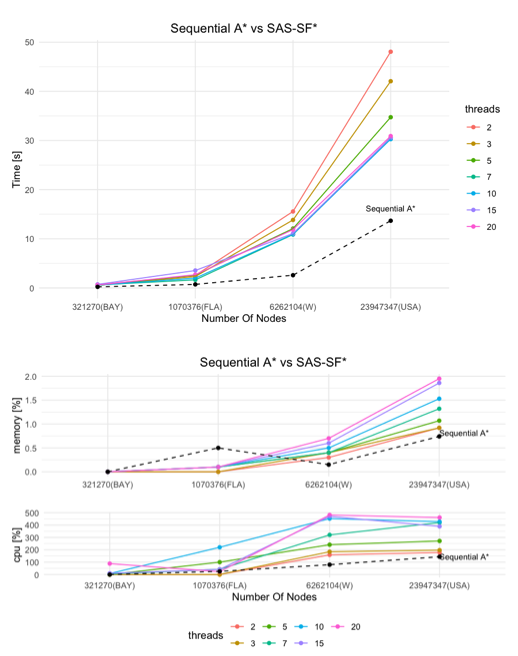
\includegraphics[width=1\linewidth]{hda/tot.png}
  \caption{HDA* overall performances}
  \label{hdatot}
\end{figure}
\begin{figure}[ht!]
  \centering
  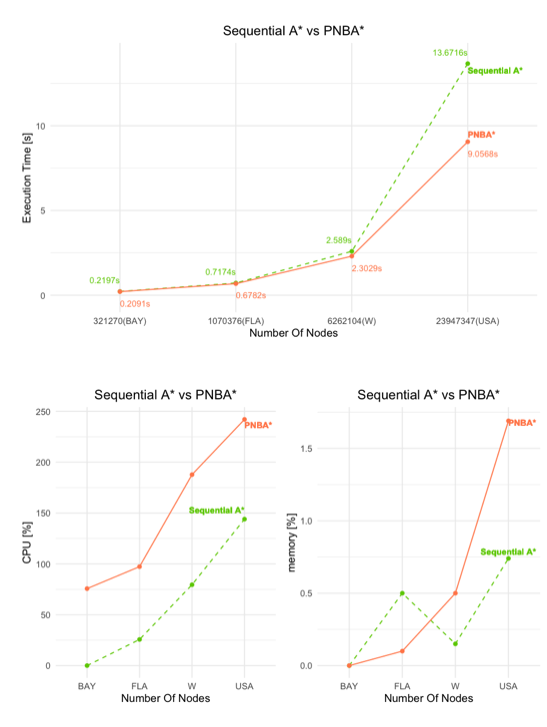
\includegraphics[width=1\linewidth]{pnba/pnba.png}
  \caption{PNBA* overall performances}
  \label{pnbatot}
\end{figure}
\begin{figure}[ht!]
  \centering
  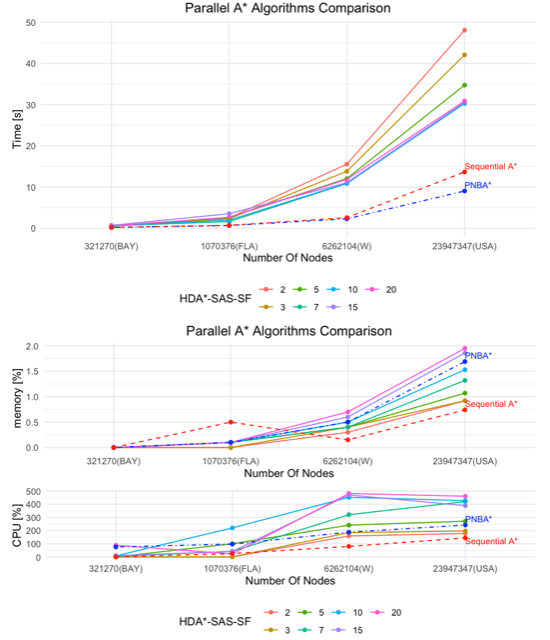
\includegraphics[width=1\linewidth]{others/allalgo.png}
  \caption{Parallel A* overall performances}
  \label{allalgo}
\end{figure}
\normalsize
\bibliography{references}
%[1] PNBA*: A parallel bidirectional heuristic search algorithm. (n.d.). Retrieved September 7, 2022, from https://homepages.dcc.ufmg.br/~chaimo/public/ENIA11.pdf
%[2] Parallel A* graph search - massachusetts institute of technology. (n.d.). Retrieved September 7, 2022, from https://people.csail.mit.edu/rholladay/docs/parallel_search_report.pdf
%[3] Heuristics. (n.d.). Retrieved September 7, 2022, from http://theory.stanford.edu/~amitp/GameProgramming/Heuristics.html
%[4] Wikimedia Foundation. (2022, August 18). A* search algorithm. Wikipedia. Retrieved September 7, 2022, from https://en.wikipedia.org/wiki/A*_search_algorithm
%[5] Proceedings of the twenty-second international joint conference ... - IJCAI. (n.d.). Retrieved September 7, 2022, from https://www.ijcai.org/Proceedings/11/Papers/105.pdf
%%%%%%%%%%%%  Supplementary Figures  %%%%%%%%%%%%
%\clearpage

%%%%%%%%%%%%%%%%   End   %%%%%%%%%%%%%%%%
%\end{multicols}  % Method B for two-column formatting (doesn't play well with line numbers), comment out if using method A
\end{document}